\begin{blocksection}
\question 
For the next 2 parts, consider that we are running the following code, in parallel, from two
distinct processes whose virtual memory specifications are the same as that of above. Both
arrays are located at page ­aligned addresses. As a note, 65536 = $2^{16}$.

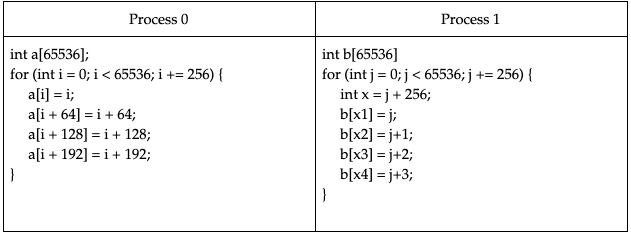
\includegraphics[width=\textwidth]{virtualmemory/ctxswitchcode}

As our computer has only a single processor, the processes must share time on the CPU. 
Thus, for each iteration of the processes’ respective for loop, the execution on this single processor follows the diagram at the top of the next page.
 A blank slot for a process means that it is not currently executing on the CPU.

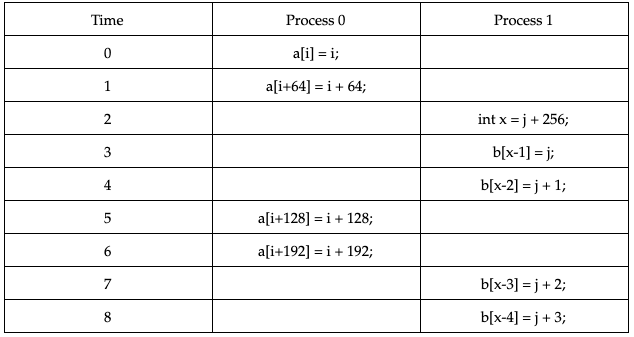
\includegraphics[width=\textwidth]{virtualmemory/ctxswitchtable}

\begin{parts}
\part
What is the TLB hit rate for executing the above code assuming that the TLB starts out cold (i.e. all entries are invalid)? 
Only consider accesses to data and ignore any effects of fetching instructions. 
You may assume that the variables i, j and x are stored in registers and therefore do not require memory accesses. 
Remember: you must flush the TLB on a context switch from one process to another!

\begin{solution}[0.5in]
50\%. The first access is a[0], which brings in the VPN translation for a[64], the next access. 
When we switch processes, the TLB will be flushed, so the first two accesses to the array b will follow the pattern miss ­hit. 
When we switch back to process 0, we access a[128] (miss because TLB empty) and a[192] (hit because brought in by a[128]). 
The execution of the second two accesses to b are also miss­ hit because the TLB is flushed in between. This pattern continues to give a hit rate of 50\%.
\end{solution}

\end{parts}


\end{blocksection}